\documentclass[12pt, a4paper]{elsarticle}

% ------------ packages -------------

\usepackage[utf8]{inputenc}
\usepackage[OT1]{fontenc}
\usepackage{graphicx}
\usepackage[english]{babel}

\usepackage{amsmath}
\usepackage{amsfonts}
\usepackage{amssymb}
\usepackage{amsthm}

\usepackage[usenames,dvipsnames]{xcolor}
\usepackage{booktabs}
\usepackage{todonotes}
\usepackage{etoolbox}
\usepackage{url}
\usepackage{tikz}
\usetikzlibrary{calc,shapes.misc,decorations}
\usetikzlibrary{decorations.pathreplacing}
%\usetikzlibrary{shapes.misc,fit}

\usepackage[bookmarks]{hyperref}

% ------------ custom defs -------------

\usepackage{mathtools}

\newtheorem{theorem}{Theorem}
\newtheorem{lemma}[theorem]{Lemma}
\newtheorem{proposition}[theorem]{Proposition}
\newtheorem{corollary}[theorem]{Corollary}

\newcommand{\reals}{\mathbb{R}}
\newcommand{\posreals}{\reals_{>0}}
\newcommand{\posrealszero}{\reals_{\ge 0}}
\newcommand{\naturals}{\mathbb{N}}

\newcommand{\mbf}[1]{\mathbf{#1}}
\newcommand{\bs}[1]{\boldsymbol{#1}}
\renewcommand{\vec}[1]{{\bs#1}}

\newcommand{\uz}{^{(0)}} % upper zero
\newcommand{\un}{^{(n)}} % upper n
\newcommand{\ui}{^{(i)}} % upper i

\newcommand{\ul}[1]{\underline{#1}}
\newcommand{\ol}[1]{\overline{#1}}

%\newcommand{\lows}{\ul{s}}
%\newcommand{\upps}{\ol{s}}

\newcommand{\Rsys}{R_\text{sys}}
\newcommand{\lRsys}{\ul{R}_\text{sys}}
\newcommand{\uRsys}{\ol{R}_\text{sys}}

\newcommand{\Fsys}{F_\text{sys}}
\newcommand{\lFsys}{\ul{F}_\text{sys}}
\newcommand{\uFsys}{\ol{F}_\text{sys}}

\def\Tsys{T_\text{sys}}

\newcommand{\E}{\operatorname{E}}
\newcommand{\V}{\operatorname{Var}}

\newcommand{\indic}{\mathbb{I}}

\newcommand{\ber}{\operatorname{Bernoulli}} 
\newcommand{\bin}{\operatorname{Binomial}}
\newcommand{\be}{\operatorname{Beta}} 
\newcommand{\bebin}{\operatorname{Beta-Binomial}} 

\def\tmax{t_\text{max}}
\def\tnow{t_\text{now}}
\def\tpnow{t^+_\text{now}}

\newcommand{\ptk}{p^k_t}

\def\yz{y\uz}
\def\yn{y\un}
%\def\yi{y\ui}
\newcommand{\yfun}[1]{y^{({#1})}}
\newcommand{\yfunl}[1]{\ul{y}^{({#1})}}
\newcommand{\yfunu}[1]{\ol{y}^{({#1})}}

\def\yl{\ul{y}}
\def\yu{\ol{y}}
\def\nl{\ul{n}}
\def\nu{\ol{n}}
\def\nktzo{\widetilde{n}\uz_{k,t}}
\def\pl{\ul{\psi}}
\def\pu{\ol{\psi}}
\def\el{\ul{\eta}}
\def\eu{\ol{\eta}}
\def\epl{\ul{\varepsilon}}
\def\epu{\ol{\varepsilon}}


\def\ykt{y_{k,t}}

\def\ykz{y\uz_k}
\def\ykn{y\un_k}

\def\yktz{y\uz_{k,t}}
\def\yktn{y\un_{k,t}}

\def\yzl{\ul{y}\uz}
\def\yzu{\ol{y}\uz}
\def\ynl{\ul{y}\un}
\def\ynu{\ol{y}\un}
\def\yil{\ul{y}\ui}
\def\yiu{\ol{y}\ui}

\def\ykzl{\ul{y}\uz_k}
\def\ykzu{\ol{y}\uz_k}
\def\yknl{\ul{y}\un_k}
\def\yknu{\ol{y}\un_k}

\def\yktzl{\ul{y}\uz_{k,t}}
\def\yktzu{\ol{y}\uz_{k,t}}
\def\yktnl{\ul{y}\un_{k,t}}
\def\yktnu{\ol{y}\un_{k,t}}

\newcommand{\ytz}[1]{y\uz_{#1,t}}
\newcommand{\ytzl}[1]{\ul{y}\uz_{#1,t}}
\newcommand{\ytzu}[1]{\ol{y}\uz_{#1,t}}

\newcommand{\ytn}[1]{y\un_{#1,t}}
\newcommand{\ytnl}[1]{\ul{y}\un_{#1,t}}
\newcommand{\ytnu}[1]{\ol{y}\un_{#1,t}}

\def\nz{n\uz}
\def\nn{n\un}
%\def\ni{n\ui}
\newcommand{\nfun}[1]{n^{({#1})}}
\newcommand{\nfunl}[1]{\ul{n}^{({#1})}}
\newcommand{\nfunu}[1]{\ol{n}^{({#1})}}

\def\nkz{n\uz_k}
\def\nkn{n\un_k}
\newcommand{\nkzfun}[1]{n\uz_{#1}}

\def\nkt{n_{k,t}}

\def\nktz{n\uz_{k,t}}
\def\nktn{n\un_{k,t}}


\def\nzl{\ul{n}\uz}
\def\nzu{\ol{n}\uz}
\def\nnl{\ul{n}\un}
\def\nnu{\ol{n}\un}
\def\nil{\ul{n}\ui}
\def\niu{\ol{n}\ui}

\def\nkzl{\ul{n}\uz_k}
\def\nkzu{\ol{n}\uz_k}
\def\nknl{\ul{n}\un_k}
\def\nknu{\ol{n}\un_k}

\def\nktzl{\ul{n}\uz_{k,t}}
\def\nktzu{\ol{n}\uz_{k,t}}
\def\nktnl{\ul{n}\un_{k,t}}
\def\nktnu{\ol{n}\un_{k,t}}

\newcommand{\ntz}[1]{n\uz_{#1,t}}
\newcommand{\ntzl}[1]{\ul{n}\uz_{#1,t}}
\newcommand{\ntzu}[1]{\ol{n}\uz_{#1,t}}

\def\taut{\tau(\vec{t})}
\def\ttau{\tilde{\tau}}
\def\ttaut{\ttau(\vec{t})}

\def\MZ{\mathcal{M}\uz}
\def\MN{\mathcal{M}\un}

\def\MkZ{\mathcal{M}\uz_k}
\def\MkN{\mathcal{M}\un_k}

\def\MktZ{\mathcal{M}\uz_{k,t}}
\def\MktN{\mathcal{M}\un_{k,t}}

\def\PZ{\Pi\uz}
\def\PN{\Pi\un}

\def\PkZ{\Pi\uz_k}
\def\PkN{\Pi\un_k}
\newcommand{\PZi}[1]{\Pi\uz_{#1}}

\def\PktZ{\Pi\uz_{k,t}}
\def\PktN{\Pi\un_{k,t}}
\newcommand{\PtZi}[1]{\Pi\uz_{#1,t}}
\newcommand{\PkZi}[1]{\Pi\uz_{k,#1}}



%\newcommand{\comments}[1]{{\small\color{gray} #1}}
\newtoggle{td}
\newcommand{\td}[1]{%
  \iftoggle{td}{%
    \todo[inline]{#1}%
  }{}%
}

\newcommand\fail[1][black]{%
  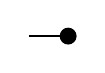
\begin{tikzpicture}
  [fail/.style={circle, draw, inner sep=0, minimum size=2mm, fill}]
    \node [fail] (c) at (0.5,0) {};
    \draw[thick] (0,0) -- (c);
  \end{tikzpicture}%
}

\newcommand\cens[1][black]{%
  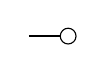
\begin{tikzpicture}
  [cens/.style={circle, draw, inner sep=0, minimum size=2mm}]
    \node [cens] (c) at (0.5,0) {};
    \draw[thick] (0,0) -- (c);
  \end{tikzpicture}%
}

\def\brcpad{0.5mm}
\newcommand\redis[4]{%
  \draw[redistr] let \p1=(#1), \p2=(#2), \p3=(#3) in ($(\x2,\y1)+(\brcpad,0)$) -- ($(\x3,\y1)+(-\brcpad,0)$) node[midway,above=5pt] {#4};
}
\newcommand\svalue[3]{%
  \path (#1) -- (#2) node[midway] {#3};
}

% ------------ options -------------

\allowdisplaybreaks

\toggletrue{td} % show todo's
%\togglefalse{td} % hide todo's

%\biboptions{longnamesfirst,angle,semicolon}


\journal{???}

\begin{document}

\begin{frontmatter}
\title{Bayesian Nonparametric Estimation\\ of Remaining Useful Life using Sets of Priors}

\author[ein]{Gero Walter}
\ead{g.m.walter@tue.nl}
\author{and others}

\address[ein]{School of Industrial Engineering, Eindhoven University of Technology, Eindhoven, NL}

\begin{abstract}
An imprecise Bayesian nonparametric approach
to system reliability with multiple types of components
for which censored observations are allowed.
This enables us to use component failure observations from a running system
to calculate its remaining useful life.
Two censoring assumptions are explored:
a minimal assumption, making use of the greater expressiveness of imprecise probability,
and the usual Kaplan-Meier-like assumption of noninformative censoring.
Both approaches are illustrated in a case study.
\end{abstract}

\begin{keyword}
System reliability \sep
Survival signature \sep
Imprecise probability \sep
Bayesian nonparametrics \sep
Prior-data conflict \sep
Censoring mechanisms
\end{keyword}
\end{frontmatter}


% ------------ manuscript -------------

\section{Introduction}

For treatment of censored observations
we see two potential approaches.
First, to obtain lower and upper system reliability bounds 
one can assume that a component either fails immediately after censoring or
continues to function during the entire time horizon.
This minimal assumption will be simple to implement but will lead to high imprecision.
Alternatively, one can assume exchangeability with other surviving components at the moment of censoring.
This approach will be more complex to accomodate but will lead to less imprecision.
Indeed, this assumption lies at the core of the Kaplan-Meier estimator \citep{1958:kaplan-meier},
and has already been adopted by \citet{2004:coolen-yan} in an imprecise probability context.\\



The \emph{survival signature} for such a system, denoted by $\Phi(l_1,\ldots,l_K)$, with $l_k=0,1,\ldots,m_k$ 
for $k=1,\ldots,K$, is defined as the probability for the event that the system functions given that \emph{precisely} $l_k$ of its 
$m_k$ components of type $k$ function, for each $k\in \{1,\ldots,K\}$ \citep{2012:survsign}.
Essentially, this creates a $K$-dimensional partition for the event $\Tsys > t$, such that $\Rsys(t) = P(\Tsys > t)$
can be calculated using the law of total probability:
\begin{align}
\label{eq:rsyswithsurvsign}
P(\Tsys > t)
 &= \sum_{l_1=0}^{m_1} \cdots \sum_{l_K=0}^{m_K} P(\Tsys > t \mid C^1_t = l_1,\ldots, C^K_t = l_K) \nonumber\\
 &  \hspace*{24ex}                        \times P\Big( \bigcap_{k=1}^K \{ C^k_t = l_k\} \Big) \nonumber\\
 &= \sum_{l_1=0}^{m_1} \cdots \sum_{l_K=0}^{m_K} \Phi(l_1, \ldots, l_K)
                                                 P\Big( \bigcap_{k=1}^K \{ C^k_t = l_k\} \Big) \,,
%                                                 \prod_{k=1}^K P(C^k_t = l_k) \,.
\end{align}
where $C^k_t \in \{0, 1, \ldots, m_k\}$ denotes
the random number of components of type $k$ functioning at time $t$.\\



Let us denote the random failure time of component number $i$ of type $k$ by $T^k_i$, $i = 1, \ldots, m_k$.
The failure time distribution can be written in terms of the cdf $F^k(t) = P(T^k_i \le t)$,
or in terms of the reliability function $R^k(t) = P(T^k_i > t) = 1 - F^k(t)$,
also known as the survival function.
For a nonparametric description of $R^k(t)$,
we consider a set of time points $t$, $t \in {\cal T} = \{t_1, \ldots, \tmax\}$.

When considering uncensored data,
at each time point $t$, the operational state of a single component of type $k$
is Bernoulli distributed (functioning: 1, failed: 0) with parameter $\ptk$, so that
\begin{align*}
P\big(\indic(T^k_i > t) = 1\big) &= \ptk\,, \\
P\big(\indic(T^k_i > t) = 0\big) &= 1 - \ptk\,,
\end{align*}
That is, $\indic(T^k_i > t) \sim \ber(\ptk)$, $i = 1, \ldots, m_k$, $t \in {\cal T}$.
The set of probabilities $\{ \ptk, t \in {\cal T}\}$
defines a discrete failure time distribution for components of type $k$ through
\begin{align*}
R^k(t_j) &= P(T^k > t_j) = p^k_{t_j},\ t_j = t_1, \ldots, \tmax\,.
\end{align*}
We can also express this failure time distribution through the probability mass function (pmf) and discrete hazard function,
\begin{align*}
f^k(t_j) &= P\big(T^k \in (t_j,t_{j+1}]\big) = p^k_{t_j} - p^k_{t_{j+1}}\,,\\ 
h^k(t_j) &= P\big(T^k \in (t_j,t_{j+1}]\mid T^k > t_j\big) % or R^k(t_{j-1}) ???
          = \frac{f^k(t_j)}{R^k(t_j)}
          = \frac{p^k_{t_j} - p^k_{t_{j+1}}}{p^k_{t_j}}\,.
\end{align*}
The time grid $\cal T$ can be chosen to be appropriately dense for the application at hand,
with the natural extension between grid points by taking $R^k(\cdot)$ to be the right continuous step function induced by the grid values,
$R^k(t) = p^k_{t_j}, t \in [t_j, t_{j+1})$,
or by taking $p^k_{t_j}$ and $p^k_{t_{j+1}}$ as upper and lower bounds for $R^k(t)$, $t \in [t_j, t_{j+1})$.

The independence assumption for components of the same type immediately implies that 
the number of functioning components of type $k$ in the system
is binomially distributed, $C^k_t = \sum_{i=1}^{m_k} \indic(T^k_i > t) \sim \bin(\ptk, m_k)$.\\



We take as prior for each $\ptk$ a Beta distribution with canonical parameters $\nz_{k,t}$ and $\yz_{k,t}$,
such that the posterior predictive probability of $l_k$ out of $m_k$ components of type $k$ functioning at time $t$
is a Beta-Binomial distribution:
\begin{align}
\lefteqn{P(C^k_t = l_k \mid s^k_t)} \nonumber \\
 &= {m_k \choose l_k} \frac{B(l_k + \nn_{k,t}\yn_{k,t}, m_k - l_k + \nn_{k,t}(1-\yn_{k,t}))}
                           {B(\nn_{k,t}\yn_{k,t}, \nn_{k,t}(1-\yn_{k,t}))} \nonumber \\
 &= {m_k \choose l_k} \frac{B(l_k + \nktz\yktz + s^k_t, m_k - l_k + \nktz(1-\yktz) + n_k - s^k_t)}
                           {B(\nktz\yktz + s^k_t, \nktz(1-\yktz) + n_k - s^k_t)} \,.
\label{eq:postpredCny}
\end{align}

%Sets of system reliability functions:
To obtain the lower and upper bound for the system reliability function $\Rsys(t)$,
we now need to minimise and maximise Equation~\eqref{eq:rsyswithsurvsign} over $\PtZi{1}, \ldots, \PtZi{K}$ for each $t$,
where the posterior predictive probabilities for $C^k_t$ are given by the Beta-Binomial pmf \eqref{eq:postpredCny}.
We therefore have
\begin{align}
\lefteqn{\lRsys(t \mid \vec{t}^1, \ldots, \vec{t}^K)} \nonumber \\
 &= \min_{\PtZi{1}, \ldots, \PtZi{K}} \Rsys(t \mid \PtZi{1}, \ldots, \PtZi{K}, \vec{t}^1, \ldots, \vec{t}^K) \nonumber \\
 &= \min_{\PtZi{1}, \ldots, \PtZi{K}} 
    \sum_{l_1=0}^{m_1} \cdots \sum_{l_K=0}^{m_K} \Phi(l_1, \ldots, l_K)
                                                 \prod_{k=1}^K P(C^k_t = l_k \mid \yktz, \nktz, s^k_t) \nonumber \\
 &= \min_{\PtZi{1}, \ldots, \PtZi{K}} 
    \sum_{l_1=0}^{m_1} \cdots \sum_{l_K=0}^{m_K} \Phi(l_1, \ldots, l_K) \times \nonumber \\ & \hspace*{12ex}
    \prod_{k=1}^K {m_k \choose l_k} \frac{B(l_k + \nn_{k,t}\yn_{k,t}, m_k - l_k + \nn_{k,t}(1-\yn_{k,t}))}
                                         {B(\nn_{k,t}\yn_{k,t}, \nn_{k,t}(1-\yn_{k,t}))} \nonumber \\
 &= \min_{\PtZi{1}, \ldots, \PtZi{K}} 
    \sum_{l_1=0}^{m_1} \cdots \sum_{l_K=0}^{m_K} \Phi(l_1, \ldots, l_K) \times \nonumber \\ & \hspace*{8ex}
    \prod_{k=1}^K {m_k \choose l_k} \frac{B(l_k + \nktz\yktz + s^k_t, m_k - l_k + \nktz(1-\yktz) + n_k - s^k_t)}
                                         {B(\nktz\yktz + s^k_t, \nktz(1-\yktz) + n_k - s^k_t)}
    \,, \label{eq:LwrSysPostA}
\intertext{which, due to results from \citet{2016:bayessurvsignsets}, can be obtained as}
 &= \sum_{l_1=0}^{m_1} \cdots \sum_{l_K=0}^{m_K} \Phi(l_1, \ldots, l_K) \times \nonumber \\ & \hspace*{8ex}
    \prod_{k=1}^K {m_k \choose l_k} \frac{B(l_k + \nktzo\yktzl + s^k_t, m_k - l_k + \nktzo(1-\yktzl) + n_k - s^k_t)}
                                         {B(\nktzo\yktzl + s^k_t, \nktzo(1-\yktzl) + n_k - s^k_t)}\,,
\label{eq:LwrSysPost}\\
 &\mathrm{where} \nonumber \\
 &\nktzo = \left\{ \begin{aligned}
   \nktzu & \quad\mbox{if}\ \yktzl < \frac{s^k_t}{n_k + m_k - 1} \vee \Big( \mathcal{L}_{\nktzu,\nktzl}(0) \ge 1 \wedge \mathcal{L}_{\nktzu,\nktzl}(m) \le 1 \Big) \\
   \nktzl & \quad\mbox{if}\ \yktzl > \frac{s^k_t + m_k - 1}{n_k + m_k - 1} \vee \Big( \mathcal{L}_{\nktzu,\nktzl}(0) \le 1 \wedge \mathcal{L}_{\nktzu,\nktzl}(m) \ge 1 \Big) \\
   & \quad\mbox{optimised otherwise}
 \end{aligned} \right. \nonumber
\end{align}
The result for $\uRsys(\cdot)$ is completely analogous.


\section{Minimal assumption for censoring}

The imprecise probability framework we are using
allows us to employ a minimal assumption for censored observations:
An upper bound for component survival is obtained by assuming that 
a censored component will not fail until the end of the considered time horizon,
i.e., by counting all censored observations as functioning when determining $s^k_t$.
A lower bound for component survival is obtained by assuming that
a censored component will fail immediately after the censoring time,
i.e., by counting all censored observations as failed when determining $s^k_t$.
These bounds encompass, in contrast to usual assumptions for censoring,
any kind of informative censoring or dependencies between censoring times and unobserved failure times. 
This can of course lead to very wide bounds, depending on the fraction of censored observations in the data.

Component survival bounds due to variation in $s^k_t$ are obtained via first-order stochastic dominance
of the Beta-Binomial distribution \eqref{eq:postpredCny} with regard to $s^k_t$,
established in Theorem~\ref{thm:s} below.
This result is completely analogous to Theorem~1 from \citet{2016:bayessurvsignsets},
which establishes first-order stochastic dominance with regard to $\yktz$.

As discussed in \citet[\S 6]{2016:bayessurvsignsets},
lower and upper bounds for the system reliability
are obtained due to monotonicity of $\Phi(\cdot)$
in each of its arguments $l_1,\ldots,l_K$.
The software implementation of \eqref{eq:LwrSysPost} in the \textsf{R}
\citep{R} package \texttt{ReliabilityTheory} \citep{2015:aslett-RT},
which assumes complete, noncensored observations,
can thus be used by suitably altering the component test data ($\vec{t}^1, \ldots, \vec{t}^K$)
for the two cases.

In Theorem~\ref{thm:s} below, indices are suppressed for readability,
and we use $\ge_{\mathrm{st}}$ to denote first-order stochastic dominance.

\begin{theorem}
  \label{thm:s}
  Let $\beta_s$ denote the Beta-Binomial distribution with probability mass function parameterised as:
  \[ p(l \mid y, n, m, s, N) \propto \frac{B(l + ny + s, m - l + n(1-y) + N - s)}{B(ny + s, n(1-y) + N - s)}, \]
  with $y, n, m,$ and $N$ fixed and unknown.
  
  Then $\beta_{\ol{s}} \ge_{\mathrm{st}} \beta_{\ul{s}} \ \forall \ \ol{s} > \ul{s} \ge 0$.
\end{theorem}

\begin{proof}%[\textbf{Proof of Theorem \ref{thm:s}, p\pageref{thm:s}}]
  \label{prf:s}
  Consider the likelihood ratio for the two Beta-Binomial distributions $\beta_{\ol{s}}$ and $\beta_{\ul{s}}$,
  \begin{align*}
    \lefteqn{\mathcal{L}(l) := \frac{p(l \mid y, n, m, \ol{s}, N)}{p(l \mid y, n, m, \ul{s}, N)}} \\
    &= \frac{B(l + n y + \ol{s}, m - l + n (1 - y) + N - \ol{s}) B(    n y + \ul{s},         n (1 - y) + N - \ul{s})}
            {B(    n y + \ol{s},         n (1 - y) + N - \ol{s}) B(l + n y + \ul{s}, m - l + n (1 - y) + N - \ul{s})} \\
    &= \frac{\Gamma(l + n y + \ol{s}) \Gamma(m - l + n (1 - y) + N - \ol{s}) \Gamma(n y + \ul{s}) \Gamma(n (1 - y) + N - \ul{s})}
            {\Gamma(l + n y + \ul{s}) \Gamma(m - l + n (1 - y) + N - \ul{s}) \Gamma(n y + \ol{s}) \Gamma(n (1 - y) + N - \ol{s})} \\
    &= \left\{ \begin{aligned}
         \frac{\prod_{x=0}^{m-1} (x + n (1 - y) + N - \ol{s})}
              {\prod_{x=0}^{m-1} (x + n (1 - y) + N - \ul{s})} &\quad\mbox{ for } l=0 \\
         \frac{\prod_{x=0}^{l-1} (x + n y + \ol{s}) \prod_{x=0}^{m-l-1} (x + n (1 - y) + N - \ol{s})}
              {\prod_{x=0}^{l-1} (x + n y + \ul{s}) \prod_{x=0}^{m-l-1} (x + n (1 - y) + N - \ul{s})} &\quad\mbox{ for } 0<l<m \\
         \frac{\prod_{x=0}^{m-1} (x + n y + \ol{s})}
              {\prod_{x=0}^{m-1} (x + n y + \ul{s})} &\quad\mbox{ for } l=m
       \end{aligned} \right.
  \end{align*}
  since $\Gamma(x+1)=x \Gamma(x)$.
  
  Thus,
  \begin{align*}
    \frac{\mathcal{L}(l+1)}{\mathcal{L}(l)} &=
      \frac{(l + n y + \ol{s}) (m - l - 1 + n (1 - y) + N - \ul{s})}
           {(l + n y + \ul{s}) (m - l - 1 + n (1 - y) + N - \ol{s})} \\
    &> 1 \quad\mbox{when}\quad \ol{s} > \ul{s} \ge 0
  \end{align*}
    
Hence, $\mathcal{L}(\cdot)$ is monotone increasing for $\ol{s} > \ul{s} \ge 0$,
so that $\beta_{\ol{s}}$ is larger than or equal to $\beta_{\ul{s}}$ in monotone likelihood ratio order
($\beta_{\ol{s}} \ge_\mathrm{lr} \beta_{\ul{s}}$).
But, $\beta_{\ol{s}} \ge_\mathrm{lr} \beta_{\ul{s}} \implies \beta_{\ol{s}} \ge_\mathrm{st} \beta_{\ul{s}}$
(\cite[Theorem 1.C.1, p.43]{shaked2007}) giving the required result.
\end{proof}

When a large part of the observations is censored,
this approach leads to high posterior imprecision,
which may easily exceed prior imprecision.
This is illustrated in ***bearing example?***


\section{Noninformative censoring assumption}

Let us first fix some notation, dropping the superscript $k$ for component types for a while.
Assuming event times and censoring times ordered separately,
we denote event times by $t_i$, $i=1, \ldots n_e$,
and censoring times by $c_i$, $i=1, \ldots n_c$,
where $n_e + n_c = n$.
The \emph{risk set} at time $t$ gives the set of units at risk at time $t$,
which is the set of observations that neither have had an event nor have been censored by time $t$,
$\{ i \mid n_i > t \} \cup \{ i \mid c_i > t \}$.
We denote the size of the risk set just before a censoring time $c_i$ by $n_{c_i}$,
% the moment of censoring of the $i$th censored observation
i.e., $n_{c_i} = \#(\{ j \mid n_j \ge c_i \} \cup \{ j \mid c_j \ge c_i \})$.
%The risk set just before the moment of censoring
%consists of these observations and the observation about to be censored.
(Note that $n_{c_i}$ includes the unit corresponding to $c_i$.)

In noninformative censoring, one assumes that
at the moment of censoring, a censored observation's unknown remaining lifetime
is exchangeable with the remaining lifetimes of all other units that were at risk at that moment. %in the current risk set.
Therefore, the rank of the unknown failure time for $c_i$ is uniformly distributed among the possible ranks $1, \ldots, n_{c_i}$,
where rank $1$ would mean that the unit actually fails before the next event or censoring time in the data set,
and rank $n_{c_i}$ would mean that the unit fails only after the last event or censoring time in the data set.
%$\max \{ t_1, \ldots, t_{n_e}, c_1, \ldots, n_{n_c}$.
Consequently, the unknown failure time may fall, with equal probability,
in each of the $n_{c_i}$ intervals formed by the censoring and event times for observations in the risk set,
setting infinity as the upper bound for the rightmost interval.

When counting the number of functioning components at a time $t$,
we can count the censored components accordingly:
As an example, assume four components having failure and censoring times $t_1 < c_1 < c_2 < t_2$.
Thus $n_{c_1} = 3$, as there is one more censoring time and one failure time after $c_1$.
We expect the component censored at $c_1$ to fail with $1/3$ probability in each of
$(c_1, c_2]$, $(c_2, t_2]$, and $(t_2, \infty)$,
that is, in each of these intervals we expect a third of a component to be functioning
due to this censored component.
Likewise, we expect the second censored component to fail with $1/2$ probability
in each of $(c_2, t_2]$ and $(t_2, \infty)$,
and so expect half a functioning component in both intervals.
%
As illustrated in Figure~\ref{fig:noninf-cens1},
we get $s_t = 2 + 1/3$ for $t \in (c_1, c_2]$,
$s_t = 1 + 1/3 + 1/2$ for $t \in (c_2, t_2]$,
and $s_t = 0 + 1/3 + 1/2$ for $t \in (t_2, \infty)$.

This approach leads to precise values for $s_t^k$
and so does not suffer from the dilation effects occuring with the minimal assumption.
The price is the fairly strong assumption of noninformative censoring;
it may be violated especially in the context of maintained systems,
where components are replaced before failing (and thus being censored)
precisely because maintenance staff believes they will fail soon.

\begin{figure}
\centering
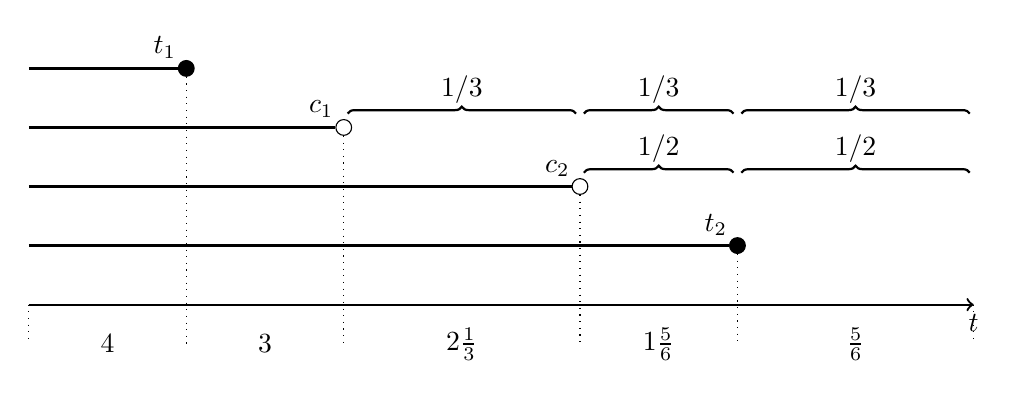
\begin{tikzpicture}
[fail/.style={circle, draw, inner sep=0, minimum size=2mm, fill=black},
 cens/.style={circle, draw, inner sep=0, minimum size=2mm},
 redistr/.style={thick, decorate, decoration={brace, raise=5pt}}]
\coordinate (tanf) at ( 0,0);
\coordinate (tend) at (12,0);
\draw[->, thick] (tanf) -- (tend) node [below] {$t$};
\node [fail] (t1) at (2,3) {};
\node [cens] (c1) at ($(t1) + (2,-0.75)$) {};
\node [cens] (c2) at ($(c1) + (3,-0.75)$) {};
\node [fail] (t2) at ($(c2) + (2,-0.75)$) {};
\foreach \obs/\lab in {t1/t_1, c1/c_1, c2/c_2, t2/t_2}
  \draw[thick] let \p1=(\obs) in (0,\y1) -- (\obs) node[above left] {$\lab$};
\redis{c1}{c1}{c2}{$1/3$}
\redis{c1}{c2}{t2}{$1/3$}
\redis{c1}{t2}{tend}{$1/3$}
\redis{c2}{c2}{t2}{$1/2$}
\redis{c2}{t2}{tend}{$1/2$}
\foreach \obs/\nam in {tanf/tanfl, t1/t1l, c1/c1l, c2/c2l, t2/t2l, tend/tendl}
  { \path let \p1=(\obs) in coordinate (\nam) at (\x1,-0.5);
    \draw[dotted] (\obs) -- (\nam);
  }
%\path (tanfl) -- (t1l) node[midway] {$4$};
\svalue{tanfl}{t1l}  {$4$}
\svalue{t1l}  {c1l}  {$3$}
\svalue{c1l}  {c2l}  {$2\frac{1}{3}$}
\svalue{c2l}  {t2l}  {$1\frac{5}{6}$}
\svalue{t2l}  {tendl}{$ \frac{5}{6}$}
\end{tikzpicture}
\caption{How to calculate $s^k_t$ based on the noninformative censoring assumption.
\fail\ denotes an observed failure, while \cens\ denotes a censored observation.
Numbers below the time axis give the resulting value of $s^k_t$.}
\label{fig:noninf-cens1}
\end{figure}

% 




% ------------ bibliography -------------

\section*{References}

\bibliographystyle{elsarticle-harv}
\bibliography{npb-cens-refs}

\end{document}
